% BEGIN PREAMBEL
\documentclass[9pt]{beamer}
\usepackage[british]{babel}
\usepackage[latin1]{inputenc}
\usepackage{multimedia}
\usepackage{amsmath,amsfonts,amssymb}
\usepackage{upgreek}
\usepackage{pgfpages}
\usepackage[version=3]{mhchem}
\usepackage{lmodern}
\usepackage{graphicx}
\usepackage{multicol}
\usepackage{color}
\usepackage{xcolor}
\usepackage{wrapfig}
\usepackage{siunitx}
\usepackage{fontspec}
\newfontfamily\ubuntu{Ubuntu}
\newcommand{\as}{\\[14pt]}
\newcommand{\s}{\\[7pt]}
\newcommand{\is}{\\[2pt]}
\newcommand{\no}{\noindent}
\newcommand{\ka}{\hspace*{0.5cm}}
\newcommand{\ma}{\hspace*{1cm}}
\newcommand{\ga}{\hspace*{1.5cm}}
\newcommand{\li}{\left|}
\newcommand{\re}{\right|}
\newcommand{\const}{\text{const.}}
\newcommand{\z}{\text}
\newcommand{\terminal}[1]{\colorbox{black}{\textcolor{white}{{\fontfamily{phv}\selectfont \scriptsize{#1}}}}}
\newcommand{\plugin}[1]{\textit{\flq#1\frq}}
\definecolor{darkcerulean}{rgb}{0.03, 0.27, 0.49}
\newcommand{\ubu}[1]{{\color{darkcerulean}\footnotesize \ubuntu #1}}
\usetheme{Boadilla}
\graphicspath{ {Pics/} }
\usecolortheme{beaver}
\useoutertheme{miniframes}
\beamertemplatenavigationsymbolsempty
\makeindex
\title[Analysis]{Discussion of the Pad Analysis}
\author[M. Reichmann]{Michael Reichmann}
\institute[\textbf{\textit{ETH}}\scalebox{.6}{\textit{Z\"{u}rich}}]{Swiss Federal Institute of Technology Zurich}
\AtBeginSection{\frame{\sectionpage}}
% END PREAMBEL
\begin{document}
% ============================
% BEGIN TITLE PAGE
% ============================
\begin{frame}
	\begin{center}
		\includegraphics[width=4cm]{SignalPeakPositions}
	\end{center}
	\begin{alertblock}{
		\begin{center}
			\textbf{Meeting \today}
		\end{center}}
		\vspace*{10pt}
		\begin{center}\small
		Michael Reichmann
		\end{center}\normalsize
	\end{alertblock}
\end{frame}
% END
% ============================
% BEGIN TABLE OF CONTENTS
% ============================
\begin{frame}[allowframebreaks]
	\frametitle{Table of contents}
	\tableofcontents   % [pausesections]
\end{frame}
% END
% ====================================================================================
% BEGIN SIGNAL PEAK POSITIONS
% ====================================================================================
\section{Signal Peak Positions}
% ============================
\subsection{Positions}
\begin{frame}
	\begin{center}
		\begin{minipage}{5.5cm}
			\centering
			\textbf{Before TCAL correction}\as
			\includegraphics[width=5.5cm]{SignalPeakPositions}
		\end{minipage}
		\hspace*{2pt}
		\begin{minipage}{5.5cm}
			\centering
			\textbf{After TCAL correction}\as
			\includegraphics[width=5.5cm]{SignalPeakPositions1}
		\end{minipage}\no\s
	\end{center}
	\begin{itemize}
		\item after correction: peak is exactly where one would expect it
		\item adding cut on the signal peak position to cut out over- and underflow bins
	\end{itemize}
\end{frame}
% new frame ============================
\begin{frame}
	\begin{center}
		\begin{minipage}{5.5cm}
			\centering
			\includegraphics[width=5.5cm]{TriggerCellVsPeakPos}
		\end{minipage}
		\hspace*{2pt}
		\begin{minipage}{5.5cm}
			\centering
			\includegraphics[width=5.5cm]{TriggerCellVsPeakPos1}
		\end{minipage}\no\s
	\end{center}
	\begin{itemize}
		\item signal peak pos supposed to be in ns
		\item after calibration we get exact timing
	\end{itemize}
\end{frame}
% new frame ============================
\subsection{Signal Vs Peak Position}
\begin{frame}
	\begin{center}
		\begin{minipage}{5.5cm}
			\centering
			\includegraphics[width=5.5cm]{SignalVsPeakPos}
		\end{minipage}
		\hspace*{2pt}
		\begin{minipage}{5.5cm}
			\centering
			\includegraphics[width=5.5cm]{SignalVsPeakPos1}
		\end{minipage}\no\s
	\end{center}
\end{frame}
% new frame ============================
\begin{frame}
	\begin{center}
		\begin{minipage}{5.5cm}
			\centering
			\includegraphics[width=5.5cm]{TriggerCellVsPeakPosSignal}
		\end{minipage}
		\hspace*{2pt}
		\begin{minipage}{5.5cm}
			\centering
			\includegraphics[width=5.5cm]{TriggerCellVsPeakPosSignal1}
		\end{minipage}\no\s
	\end{center}
	\begin{itemize}
		\item with eventwise pedestal correction
	\end{itemize}
\end{frame}
% END
% ====================================================================================
% BEGIN FORC 
% ====================================================================================
\section{FORC (Fast OR Coincidence)}
% ============================
\subsection{Positions}
\begin{frame}
	\begin{center}
		\begin{minipage}{5.5cm}
			\centering
			\includegraphics[width=5.5cm]{FORCTiming}
		\end{minipage}
		\hspace*{2pt}
		\begin{minipage}{5.5cm}
			\centering
			\includegraphics[width=5.5cm]{FORCTiming1}
		\end{minipage}\no\s
	\end{center}
	\begin{itemize}
		\item expect FORC to be flat and in between \SI{17}{ns} 
		\begin{itemize}
			\item trigger on coinc between scintillator (\SI{5}{ns}) and FORC (\SI{17}{ns})
		\end{itemize}
	\end{itemize}
\end{frame}
% ============================
\subsection{Trigger Cell vs FORC}
\begin{frame}
	\begin{center}
		\begin{minipage}{5.5cm}
			\centering
			\includegraphics[width=5.5cm]{TriggerCellVsFORC}
		\end{minipage}
		\hspace*{2pt}
		\begin{minipage}{5.5cm}
			\centering
			\includegraphics[width=5.5cm]{TriggerCellVsFORC1}
		\end{minipage}\no\s
	\begin{itemize}
		\item band is \SI{17}{ns} thick as expected
	\end{itemize}
	\end{center}
\end{frame}
% ============================
\subsection{Trigger Cell vs FORC - Full Range High Rate}
\begin{frame}
	\begin{center}
		\includegraphics[width=6.5cm]{TriggerCellVsFORCFullRange}
	\end{center}
	\begin{itemize}
		\item sub-bands separated by \SI{25}{ns} and \SI{17}{ns} thick as well
		\item use as cut for hits in other buckets
	\end{itemize}
\end{frame}
% END
% ====================================================================================
% BEGIN SIGNAL PEAK POSITIONS
% ====================================================================================
\section{Pulse Height}
% ============================
\subsection{Signal vs Trigger Cell}
\begin{frame}
	\begin{center}
		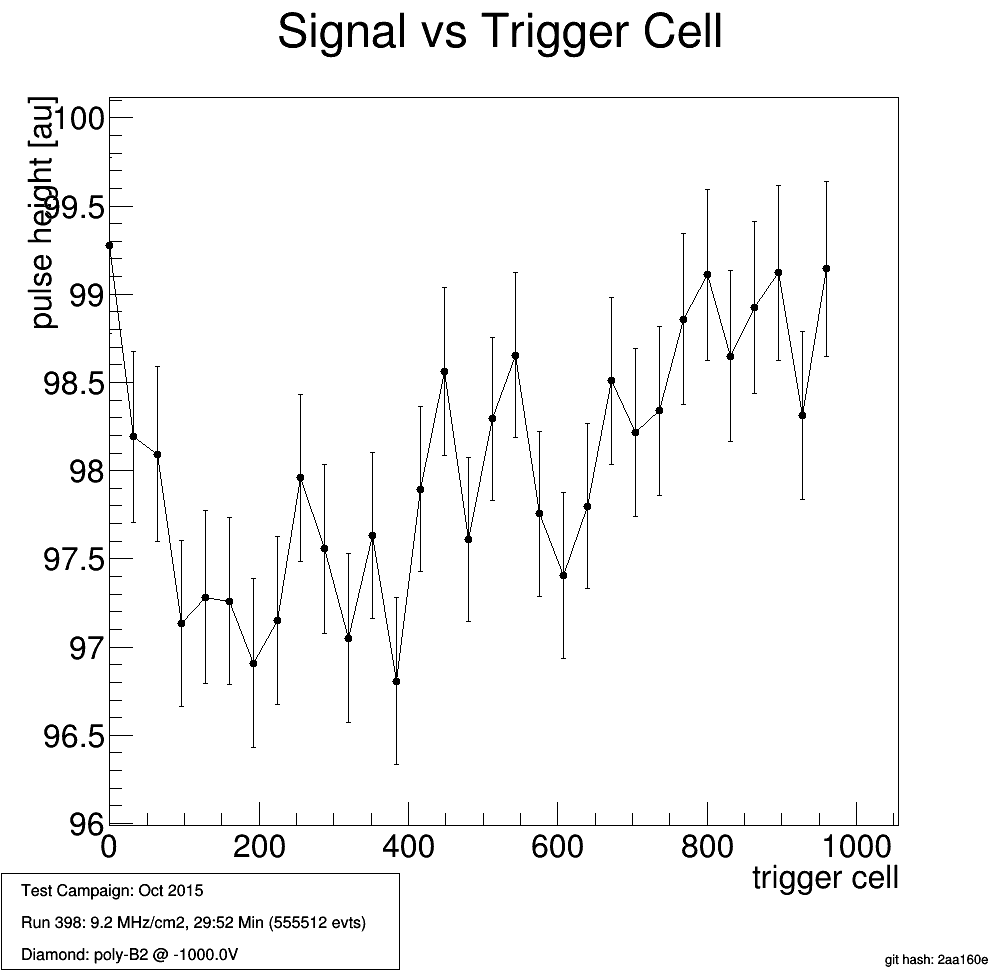
\includegraphics[width=5.5cm]{SignalVsTriggerCell}
	\end{center}
	\begin{itemize}
		\item Signal dependent on trigger cell
	\end{itemize}
\end{frame}
% ============================
\subsection{Signal vs Trigger Cell}
\begin{frame}
	\begin{center}
		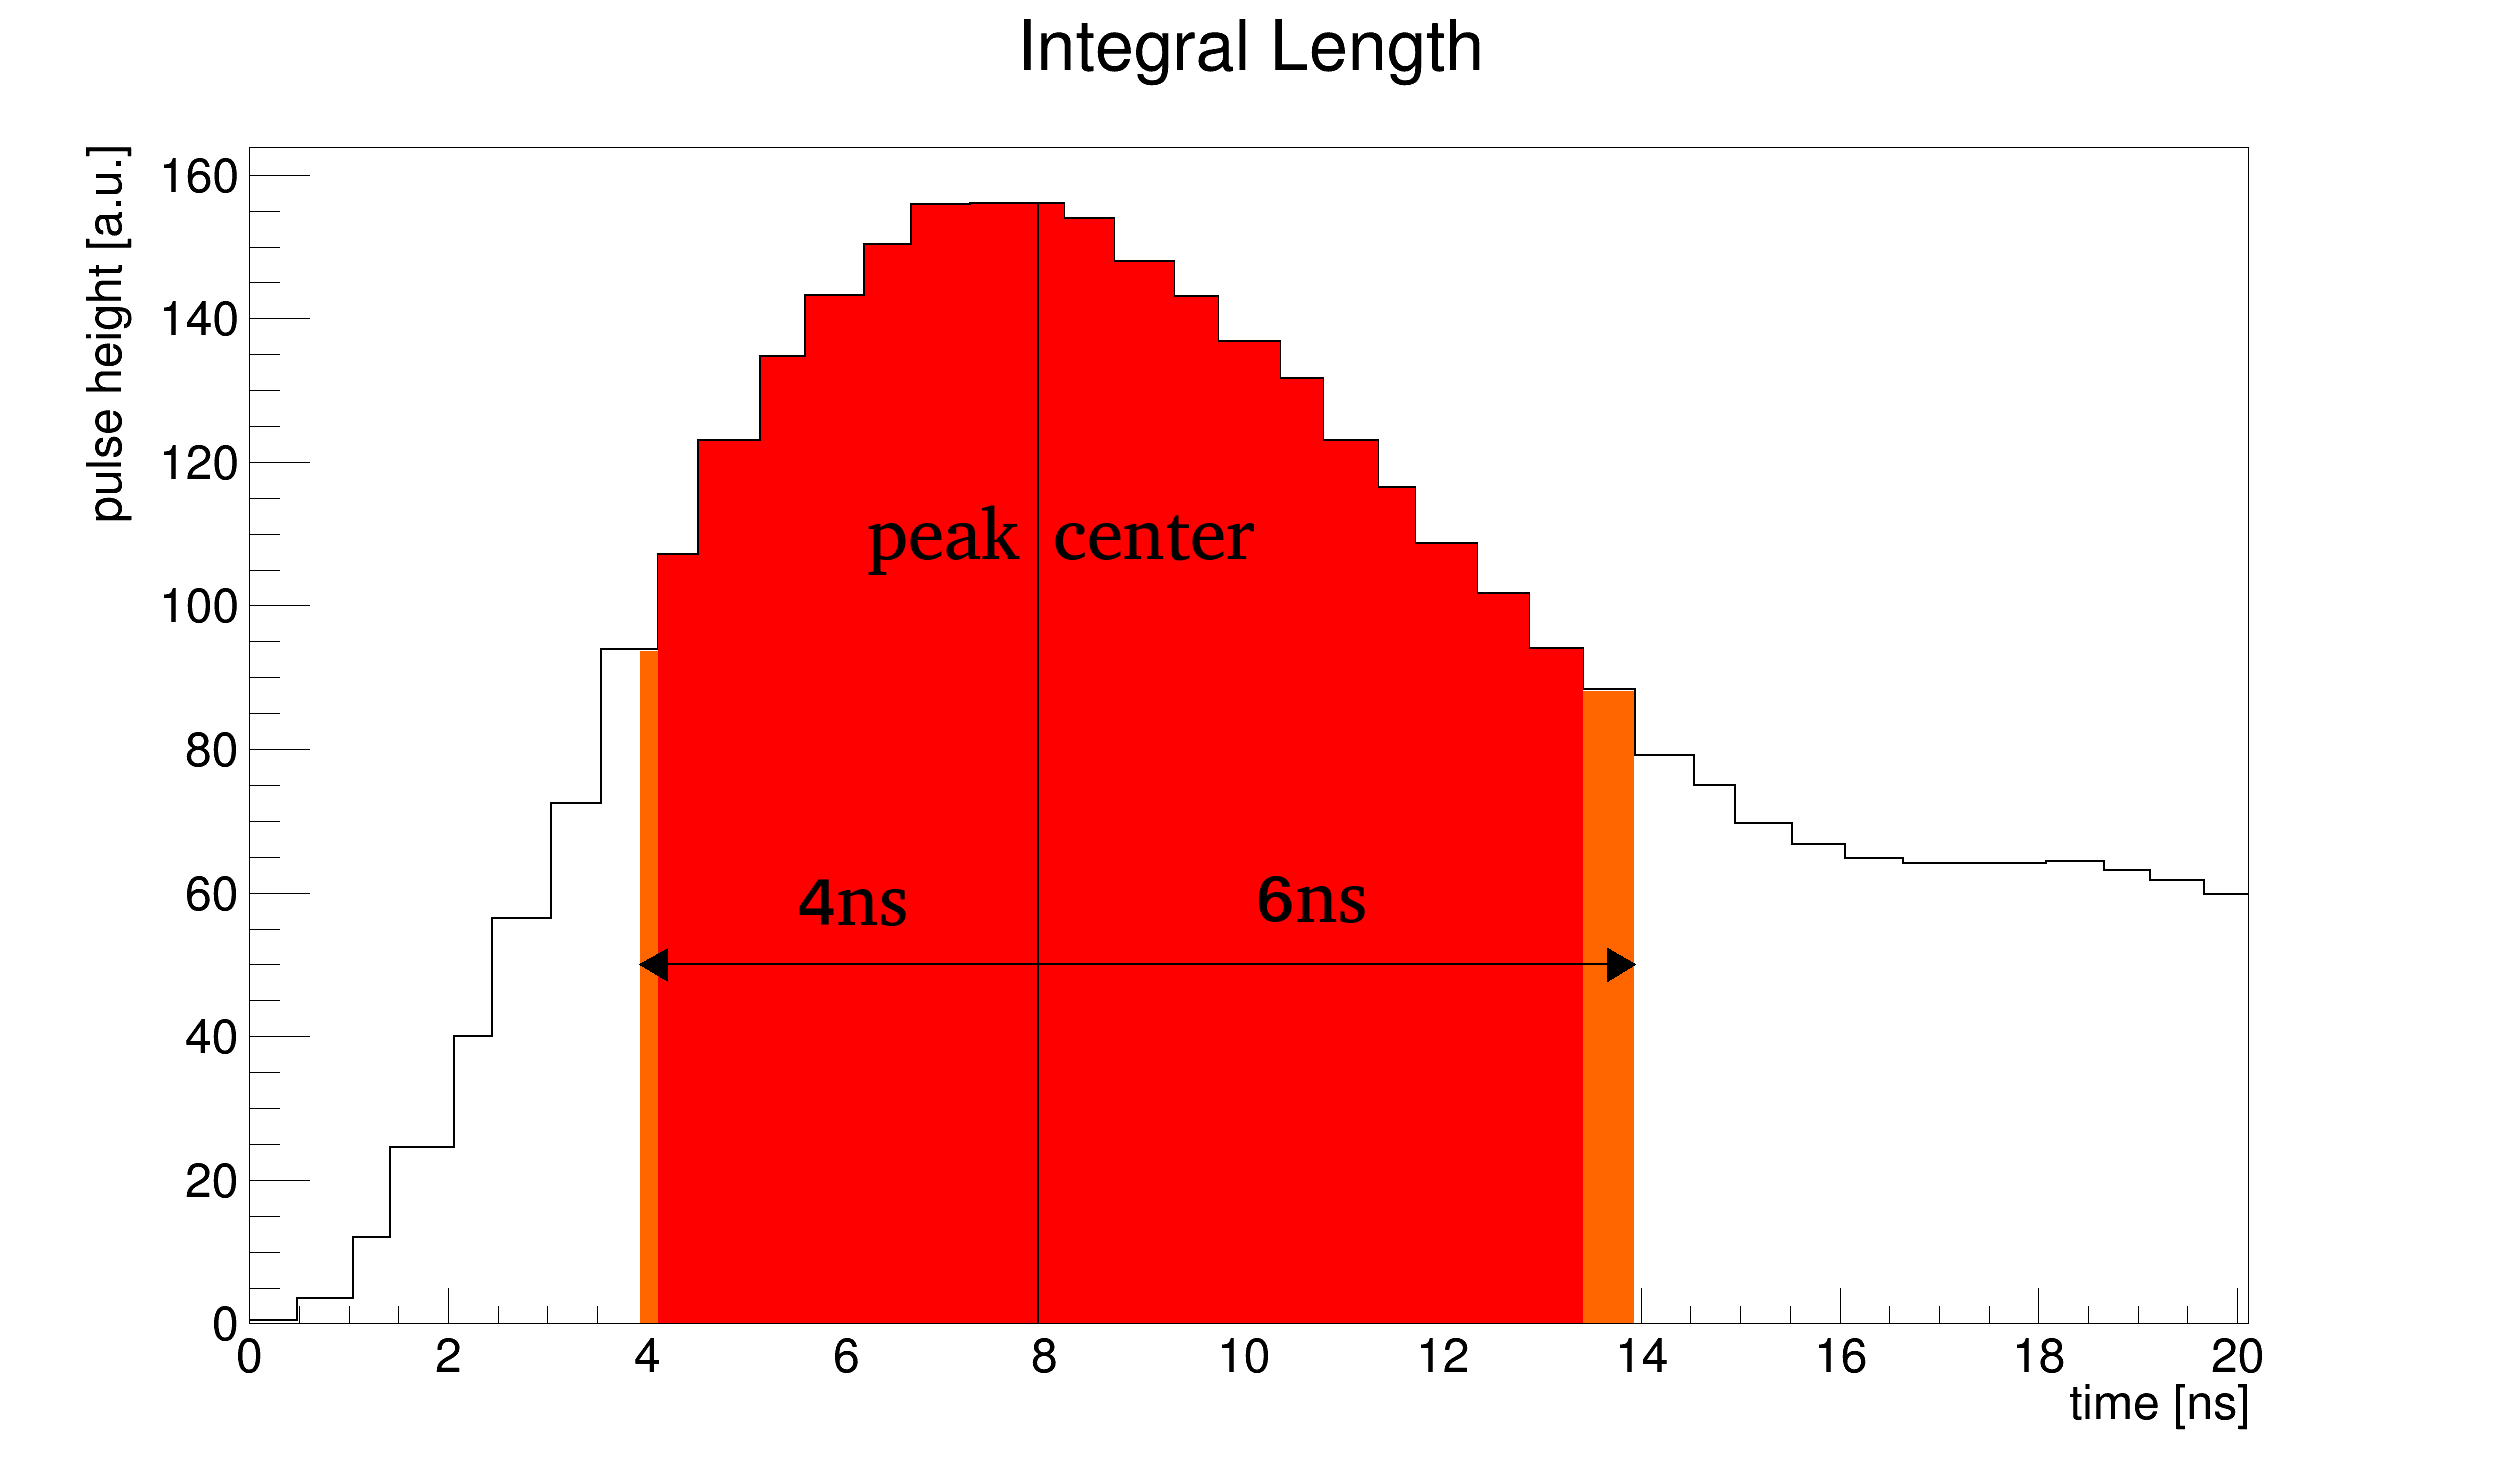
\includegraphics[width=5.5cm]{IntegralLength}
	\end{center}
	\begin{itemize}
		\item Length change within $10\%$
	\end{itemize}
\end{frame}
% END
% ====================================================================================
% BEGIN CONCLUSION
% ====================================================================================
\section{Conclusion}
% ============================
\begin{frame}
	\frametitle{Conclusion}
	\begin{minipage}[c][0.6\textheight]{\textwidth}
		\begin{itemize}
			\setlength{\itemsep}{\fill}
			\item DRS4 time calibration returns exact timing of the signal
			\begin{itemize}
				\item fixes signal peak timing
				\item fixes FORC timing
			\end{itemize}
			\item time calibration is not perfect yet
			\begin{itemize}
				\item still small dependence on the trigger cell
			\item see expected behaviour of the pulse height as function of peak pos
			\end{itemize}
			\item adding cut on signal peak timing
			\item signal dependence on trigger cell not yet fixed
		\end{itemize}
	\end{minipage}
\end{frame}
% END 
% DOCUMENT END
\end{document}

